  %%%%%%%%%%%%%%%%%%%%%%%%%%%%%%%%%%%%%%% -*- coding: utf-8; mode: latex -*- %%
  %
%%%%%                         CHAPTER
 %%%
  %

% $Id: 2200-irure-dolor.tex,v 1.1 2007/11/23 09:52:42 david Exp $
% $Log: 2200-irure-dolor.tex,v $
% Revision 1.1  2007/11/23 09:52:42  david
% *** empty log message ***
%
%

  %%%%%%%%%%%%%%%%%%%%%%%%%%%%%%%%%%%%%%%%%%%%%%%%%%%%%%%%%%%%%%%%%%%%%%%%%%%%%
  %
%%%%%                     HEAD MATTER
 %%%
  %

\chapter{Namespace Concurrency Control}
%\addcontentsline{lof}{chapter}{\thechapter\quad Irure Dolor}
%\addcontentsline{lot}{chapter}{\thechapter\quad Irure Dolor}
\label{ch:Locking}

%\begin{quotation}
%  {\small\it Neque porro quisquam est qui dolorem ipsum quia dolor sit amet, consectetur, adipisci velit...}
%
%{\small\it -- Cerico}
%\end{quotation}

\section{Namespace Concurrency Control in GFS}

\subsection{Namespace Structure}
Unlike traditional file systems, GFS doesn't have a per-directory data structure, which means that it doesn't support listing all files in a directory (i.e, \textit{ls} in POSIX), nor aliasing for the same file or directory (i.e, hard or symbolic links). Instead, with prefix compression, GFS represents the namespace as a lookup table mapping full pathnames to metadata logically, which means that the full pathnames are similar to the hash keys in a hash table.

\subsection{Namespace Concurrency Control}
Each node (either an absolute directory name or an absolute file name) in the namespace tree will be associated a \textit{read-write} lock. To prevent deadlock, locks are acquired in a \textit{consistent total order}: first ordered by level, then ordered lexicographically within the same level~\cite{ghemawat2003google}.

\noindent One benefit for the locking scheme in GFS is that it allows concurrent mutations for different files/directories within the same directory. 

\begin{figure}[ht]
	\centering
	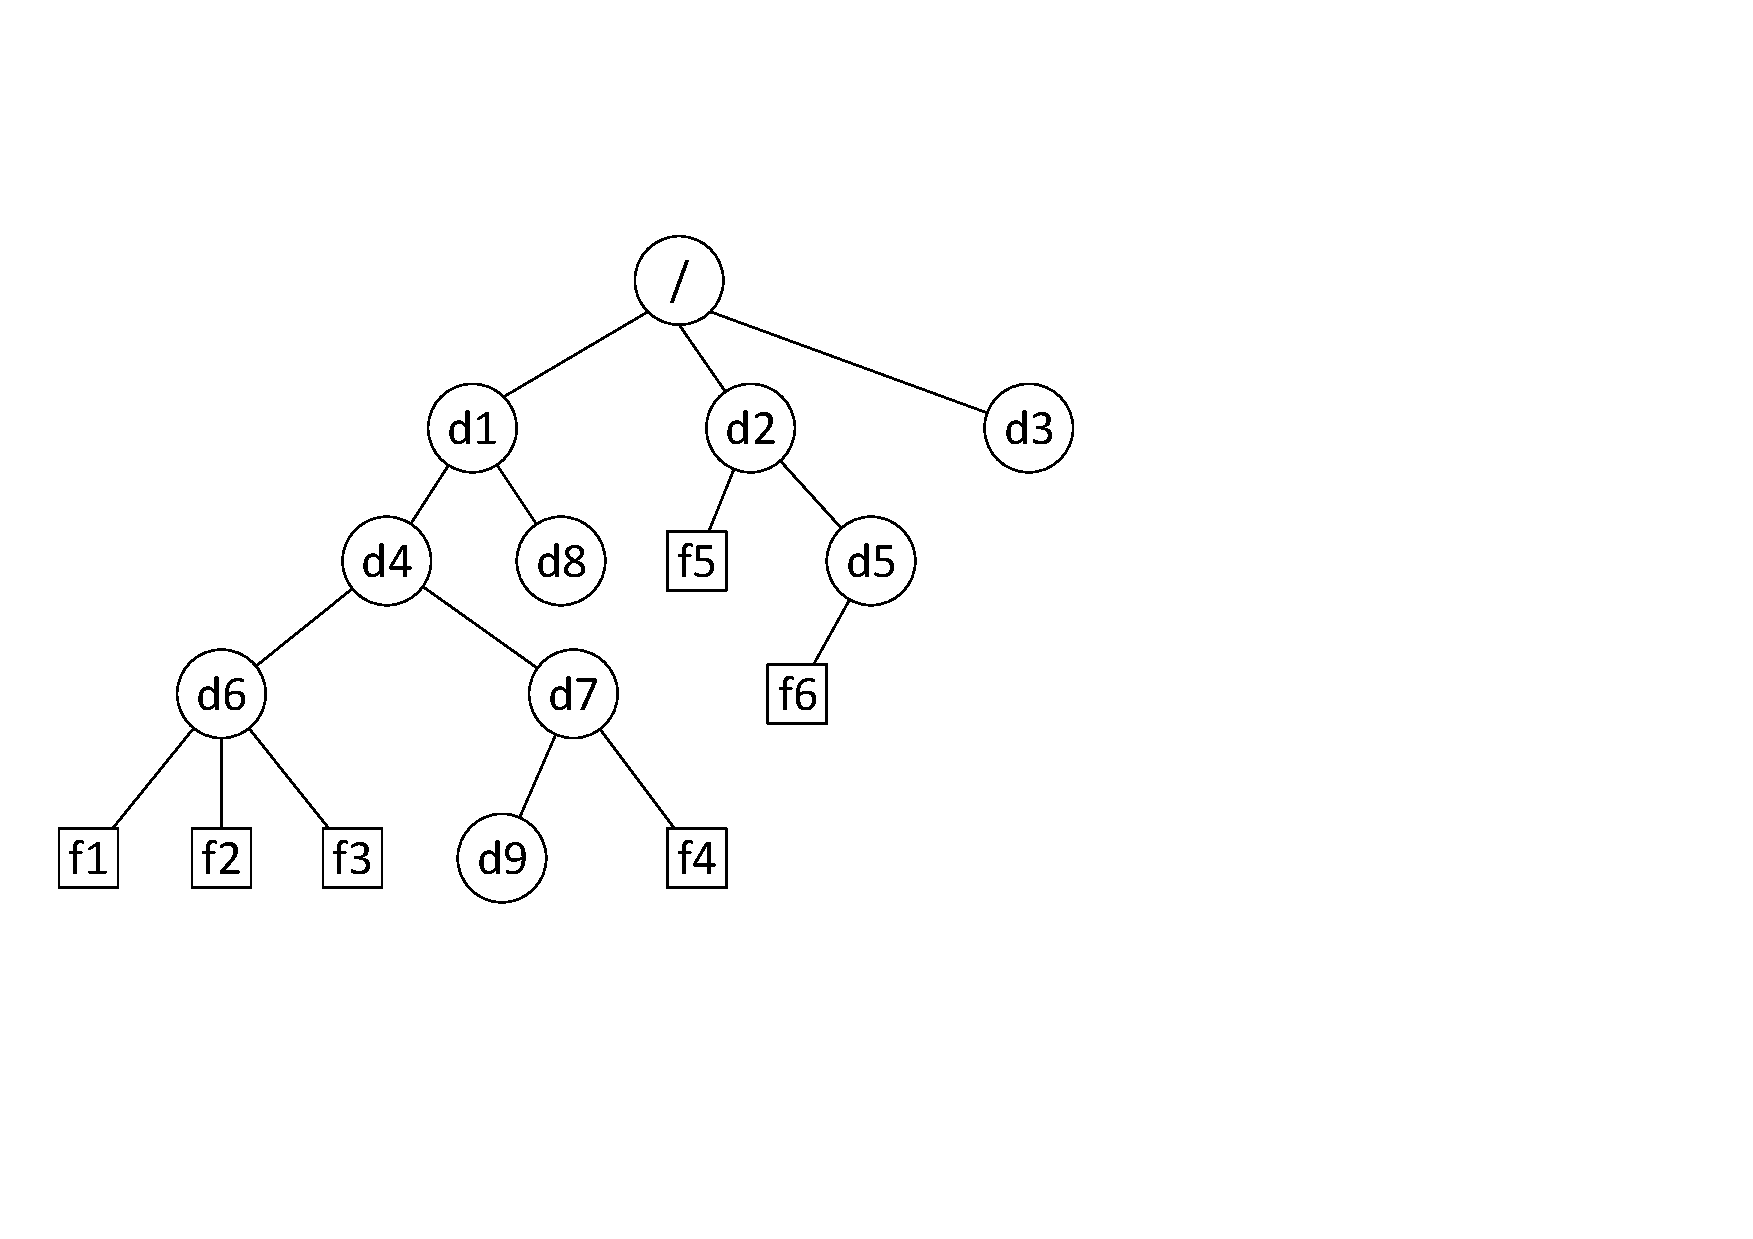
\includegraphics[scale=0.7]{figs/gfstree.pdf}
	\caption{A Graphical Tree Representation for the Namespace in GFS}
	\label{fig:gfsTree}
\end{figure}

\noindent For example, suppose that we have a graphical tree representation for the namespace in GFS as shown in Figure~\ref{fig:gfsTree}. Concurrently, we have five operations involving files \textit{f1, f2, f3, f4} and directory \textit{d9}. As we can see from Table~\ref{table:gfsLock1}, there are no conflicting locks (\textit{Read-Write and Write-Write}), all these five operations are all allowed to happen concurrently.

\begin{table}
	\centering
    \begin{tabular}{|l|c|c|c|c|c|}
    	\hline
    	\textbf{\textit{Total Order Locks}}            & \textbf{Operation1} & \textbf{Operation2} & \textbf{Operation3} & \textbf{Operation4} & \textbf{Operation5} \\ \hline
    	\textbf{\color{red}/ }           & Read1      & Read2      & Read3      & Read4      & Read5      \\ \hline
    	/\textbf{\color{red}d1}          & Read1      & Read2      & Read3      & Read4      & Read5      \\ \hline
    	/d1/\textbf{\color{red}d4}       & Read1      & Read2      & Read3      & Read4      & Read5      \\ \hline
    	/d1/d4/\textbf{\color{red}d6}    & Read1      & Read2      & Read3      & ~          & ~          \\ \hline
    	/d1/d4/\textbf{\color{red}d7}    & ~          & ~          & ~          & Read4      & Read5      \\ \hline
    	/d1/d4/d6/\textbf{\color{red}f1} & Write1     & ~          & ~          & ~          & ~          \\ \hline
    	/d1/d4/d6/\textbf{\color{red}f2} & ~          & Write2     & ~          & ~          & ~          \\ \hline
    	/d1/d4/d6/\textbf{\color{red}f3} & ~          & ~          & Write3     & ~          & ~          \\ \hline
    	/d1/d4/d7/\textbf{\color{red}d9} & ~          & ~          & ~          & Write4     & ~     \\ \hline
    	/d1/d4/d7/\textbf{\color{red}f4} & ~          & ~          & ~          & ~          & Write5          \\ \hline
    \end{tabular}
	\caption{Concurrent Mutations within for different files/directories and Related Read-Write Lock Sets}
	\label{table:gfsLock1}
\end{table}

\noindent Since operations will be serialized properly when trying to obtain conflict locks(\textit{Read-Write and Write-Write}), concurrent mutations on the same file/directory will be prevented.

\begin{table}[ht]
	\centering
	\begin{tabular}{|l|c|c|}
		\hline
		\textbf{\textit{Total Order Locks}}             & \textbf{Operation1} & \textbf{Operation2}                    \\ \hline
		\textbf{\color{red}/}             & Read1      & Read2                         \\ \hline
		/\textbf{\color{red}d1}           & Read1      & Read2                         \\ \hline
		/\textbf{\color{red}d3}           & Read1      & ~                             \\ \hline
		/d1/\textbf{\color{red}d8}        & Write1     & Read2 \textbf{(Conflicts with Write1)} \\ \hline
		/d3/\textbf{\color{red}d8}       & Write1     & ~                             \\ \hline
		/d1/d8/\textbf{\color{red}Qi.txt} & ~          & Write2                        \\ \hline
	\end{tabular}
	\caption{Serialized Concurrent Mutations and Conflict Locks}
	\label{table:gfsLock2}
\end{table}

\noindent For example, if there are another two concurrent operations. \textit{Operation 1} wants to snapshot directory \textit{d8} to be under directory \textit{d3}, but \textit{Operation 2} wants to create a new file \textit{Qi.txt} under directory \textit{d8}. Table~\ref{table:gfsLock2} shows how conflict locks prevent the new file \textit{Qi.txt} being created when directory \textit{d8} is being snapshotting.

\noindent In sum, GFS trades off common file system requirements for this namespace locking scheme with nice concurrency control properties.
  %%%%%%%%%%%%%%%%%%%%%%%%%%%%%%%%%%%%%%%%%%%%%%%%%%%%%%%%%%%%%%%%%%%%%%%%%%%%%
  %
%%%%%                        FIRST SECTION
 %%%
  %

\section{Namespace Concurrency Control in HDFS}

\subsection{Namespace Structure}

Unlike GFS, the interface to HDFS is patterned after UNIX, and it support POSIX like commands (e.g, \textit{ls, mkdir, rm, cp, chown}) to the common file system. The namespace of HDFS is structured as a hierarchy of files and directories. Files and directories are represented on the NameNode by \textit{INodes} with attributes like permissions, modification and access times, namespace and disk space quotas~\cite{borthakur2008hdfs}. Each file is represented by an \textit{INodeFile} object, each directory is represented by an \textit{INodeDirectory}, and each symbolic link is represented by an \textit{INodeSymlink object}. Figure~\ref{fig:inodeuml} shows the Namespace INode Structure in UML diagram with major attributes.

\begin{figure}[h]
	\centering
	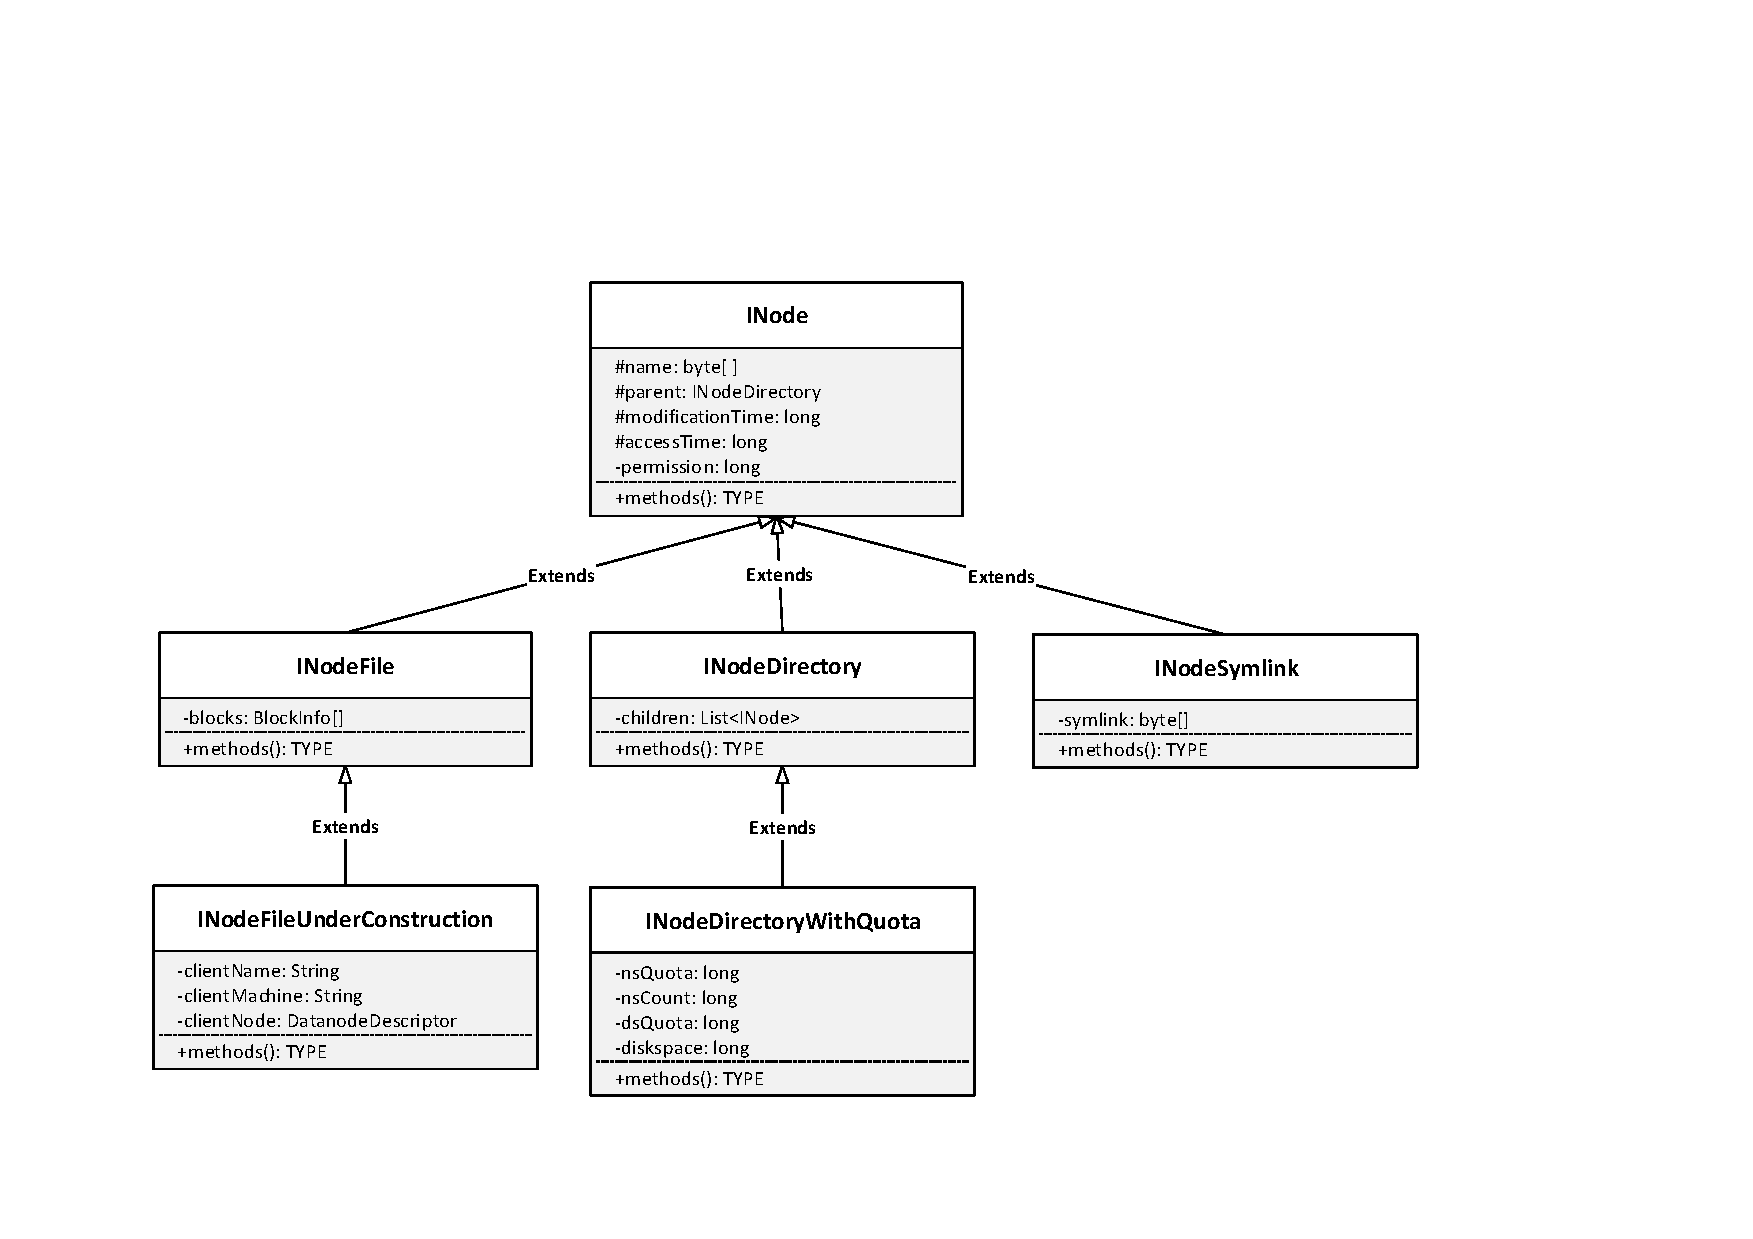
\includegraphics[width=\linewidth]{figs/INodeUML.pdf}
	\caption{The Namespace INode Structure in HDFS}
	\label{fig:inodeuml}
\end{figure}

\subsection{Namespace Concurrency Control}

\noindent The hierarchical INode structure makes HDFS not possible to adopt the namespace locking scheme from GFS. In order to support POSIX like operations (list files, set quotas, create symbolic links), INodeFiles, INodeDirectories and INodeSymlink objects are semantically related to each other, rather than just logical representation.

\noindent For example, suppose that HDFS adopts the namespace locking scheme in GFS. An INodeDirectory \textit{D3} with quota \textit{1} which only allows 1 more INode to be created inside it. Concurrently, there are four operations try to create an INodeFile inside \textit{D3}. All of them put a read lock on \textit{D3} first. Finding that the quota is 1, they then put a write lock on the file and create it under the directory. Finally four files are created under \textit{D3} but it violates the quota. See Figure~\ref{fig:hdfsquota}.

\begin{figure}[h]
	\centering
	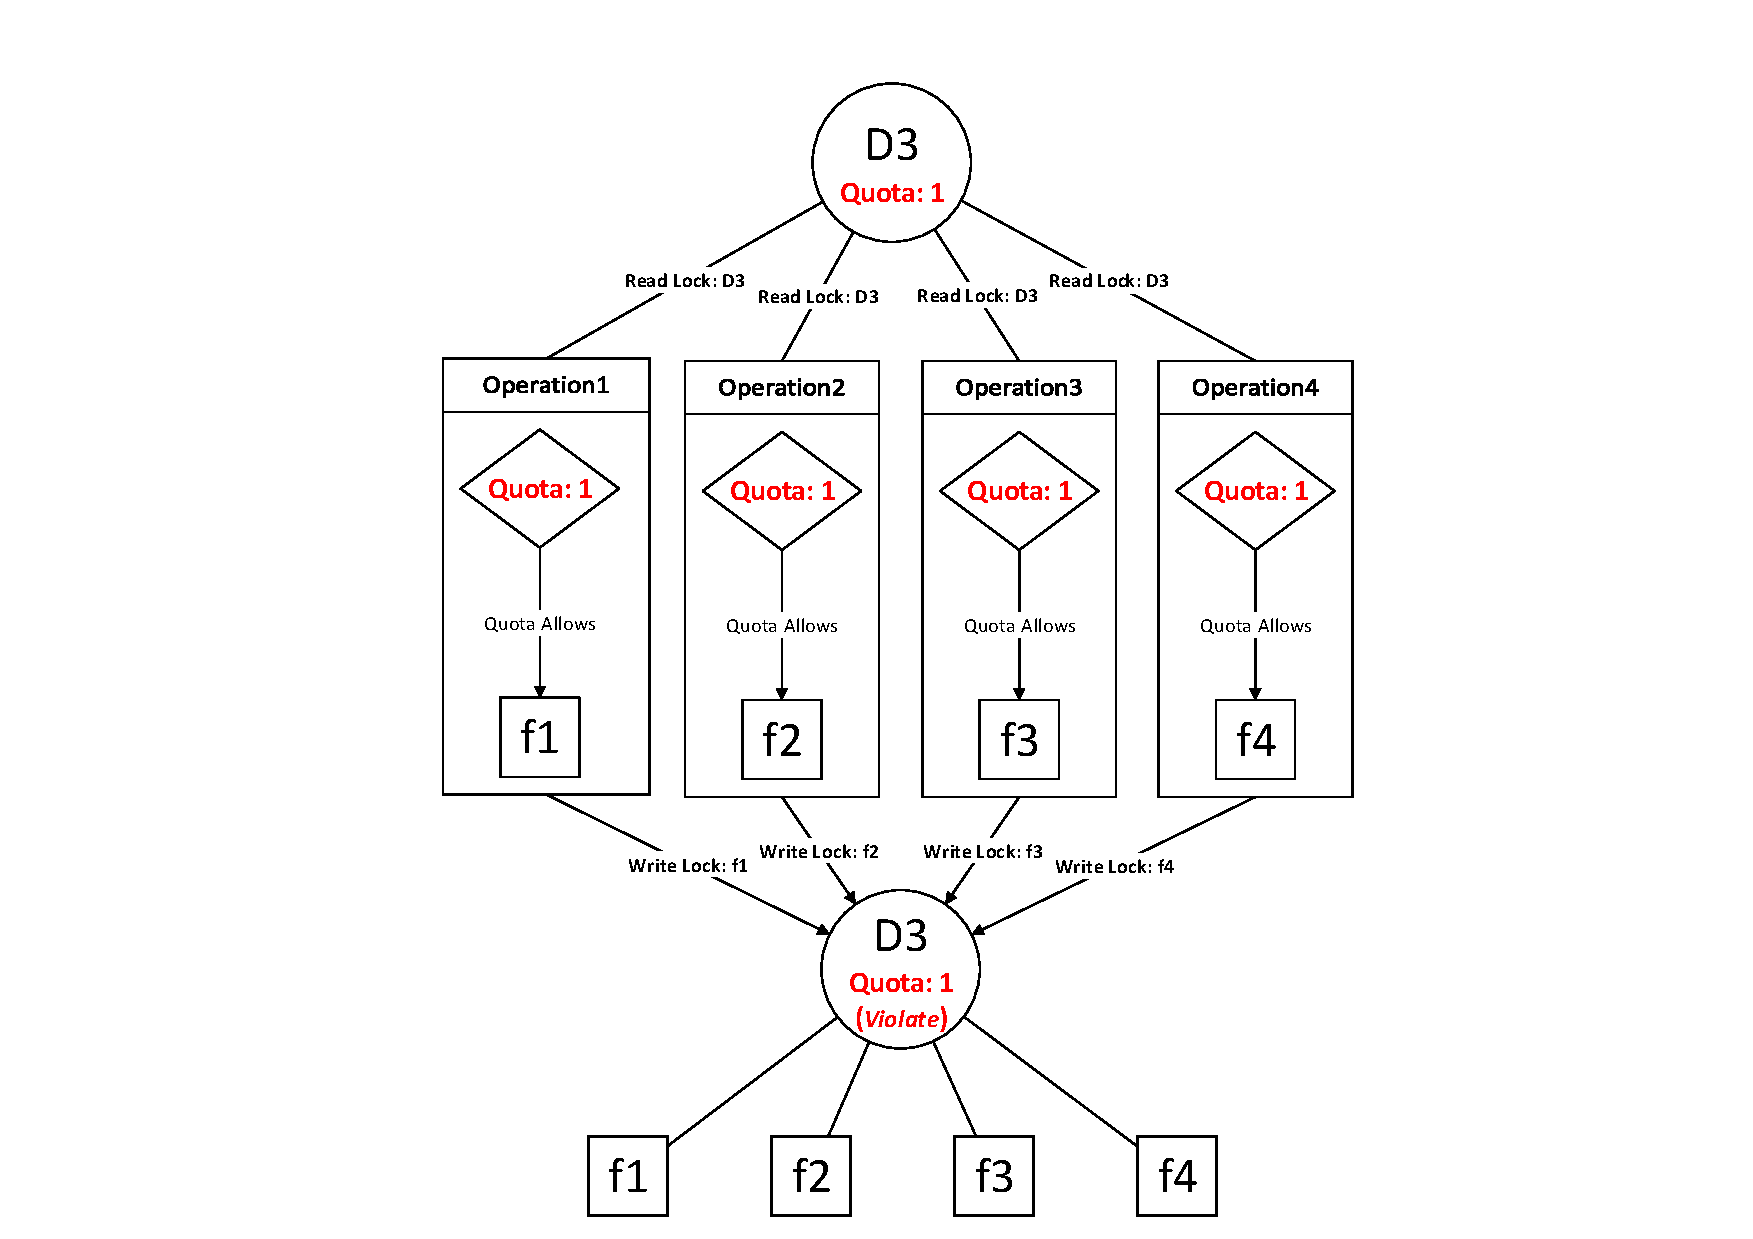
\includegraphics[scale=0.7]{figs/hdfsquota.pdf}
	\caption{Violation in Quota Semantic}
	\label{fig:hdfsquota}
\end{figure}

\noindent One way to solve this consistency problem is to synchronize all the related attributes among different threads under proper semantic group. However, it complicates the namespace design and is not realistic. Therefore, to protect the namespace among parallel running threads, a global read/write lock (fsLock in \textit{FSNamesystem} - \textit{ReentrantReadWriteLock} in java language) is used to maintain the atomicity of the namespace. We call it \textit{system-level lock}.

\noindent HDFS categorizes the metadata operations into \textit{read operations} and \textit{write operations}. Concurrent threads to access the namespace for read operations are allowed, but it restricts a single thread to namespace for write operations. Therefore, all concurrent readers get the same view of the mutated data reflected by completed writes. We call it \textit{Strong Consistency Semantics} in HDFS. (But it is still weaker than the standard POSIX consistency model since it trades some POSIX requirements for performance in terms of data coherency~\cite{white2012hadoop})

\subsection{Bottleneck}

\noindent Although the namespace is kept in-memory for fast operations, the system-level lock is still the bottleneck in NameNode under high workload pressure. Here we analyze the Remote Procedure Call (RPC) for namespace operations between clients and NameNode. See Figure~\ref{fig:nnRPC} for the process:

\begin{enumerate}[noitemsep]
	\item Client makes an RPC request to NameNode RPC server, like \textit{mkdir}.
	\item The listener thread in NameNode RPC server accepts this request.
	\item The Reader, child thread of Listener, processes the request and makes it as a Call object stored in the Call Queue, waiting for the handling.
	\item One of the handlers gets a Call object (\textit{mkdir}) from the queue. As \textit{mkdir} belongs to write operation, the handler takes a write lock on the namespace.
	\item After taking the write lock, a new directory will be created in the namespace within NameNode.
	\item The modification record needs to be synchronized to the editlogs.
	\item Release the write lock.
	\item The callback is returned to the Responder thread.
	\item The client get the result for this operation (either success or fail).
\end{enumerate}

\noindent As we can see, any of the steps above may become the bottle. But in step 6, while the entire namespace is protected by the system-level lock, the modification record needs to be saved into the editlogs. Since the editlogs are written into the physical hard drives sequentially, the more syn edit to be handled, the slower it will be for the responder to return the callback. The system-level lock won't be released during this process, so the throughput will be decreased greatly during heavy workload.

\begin{figure}[h]
	\centering
	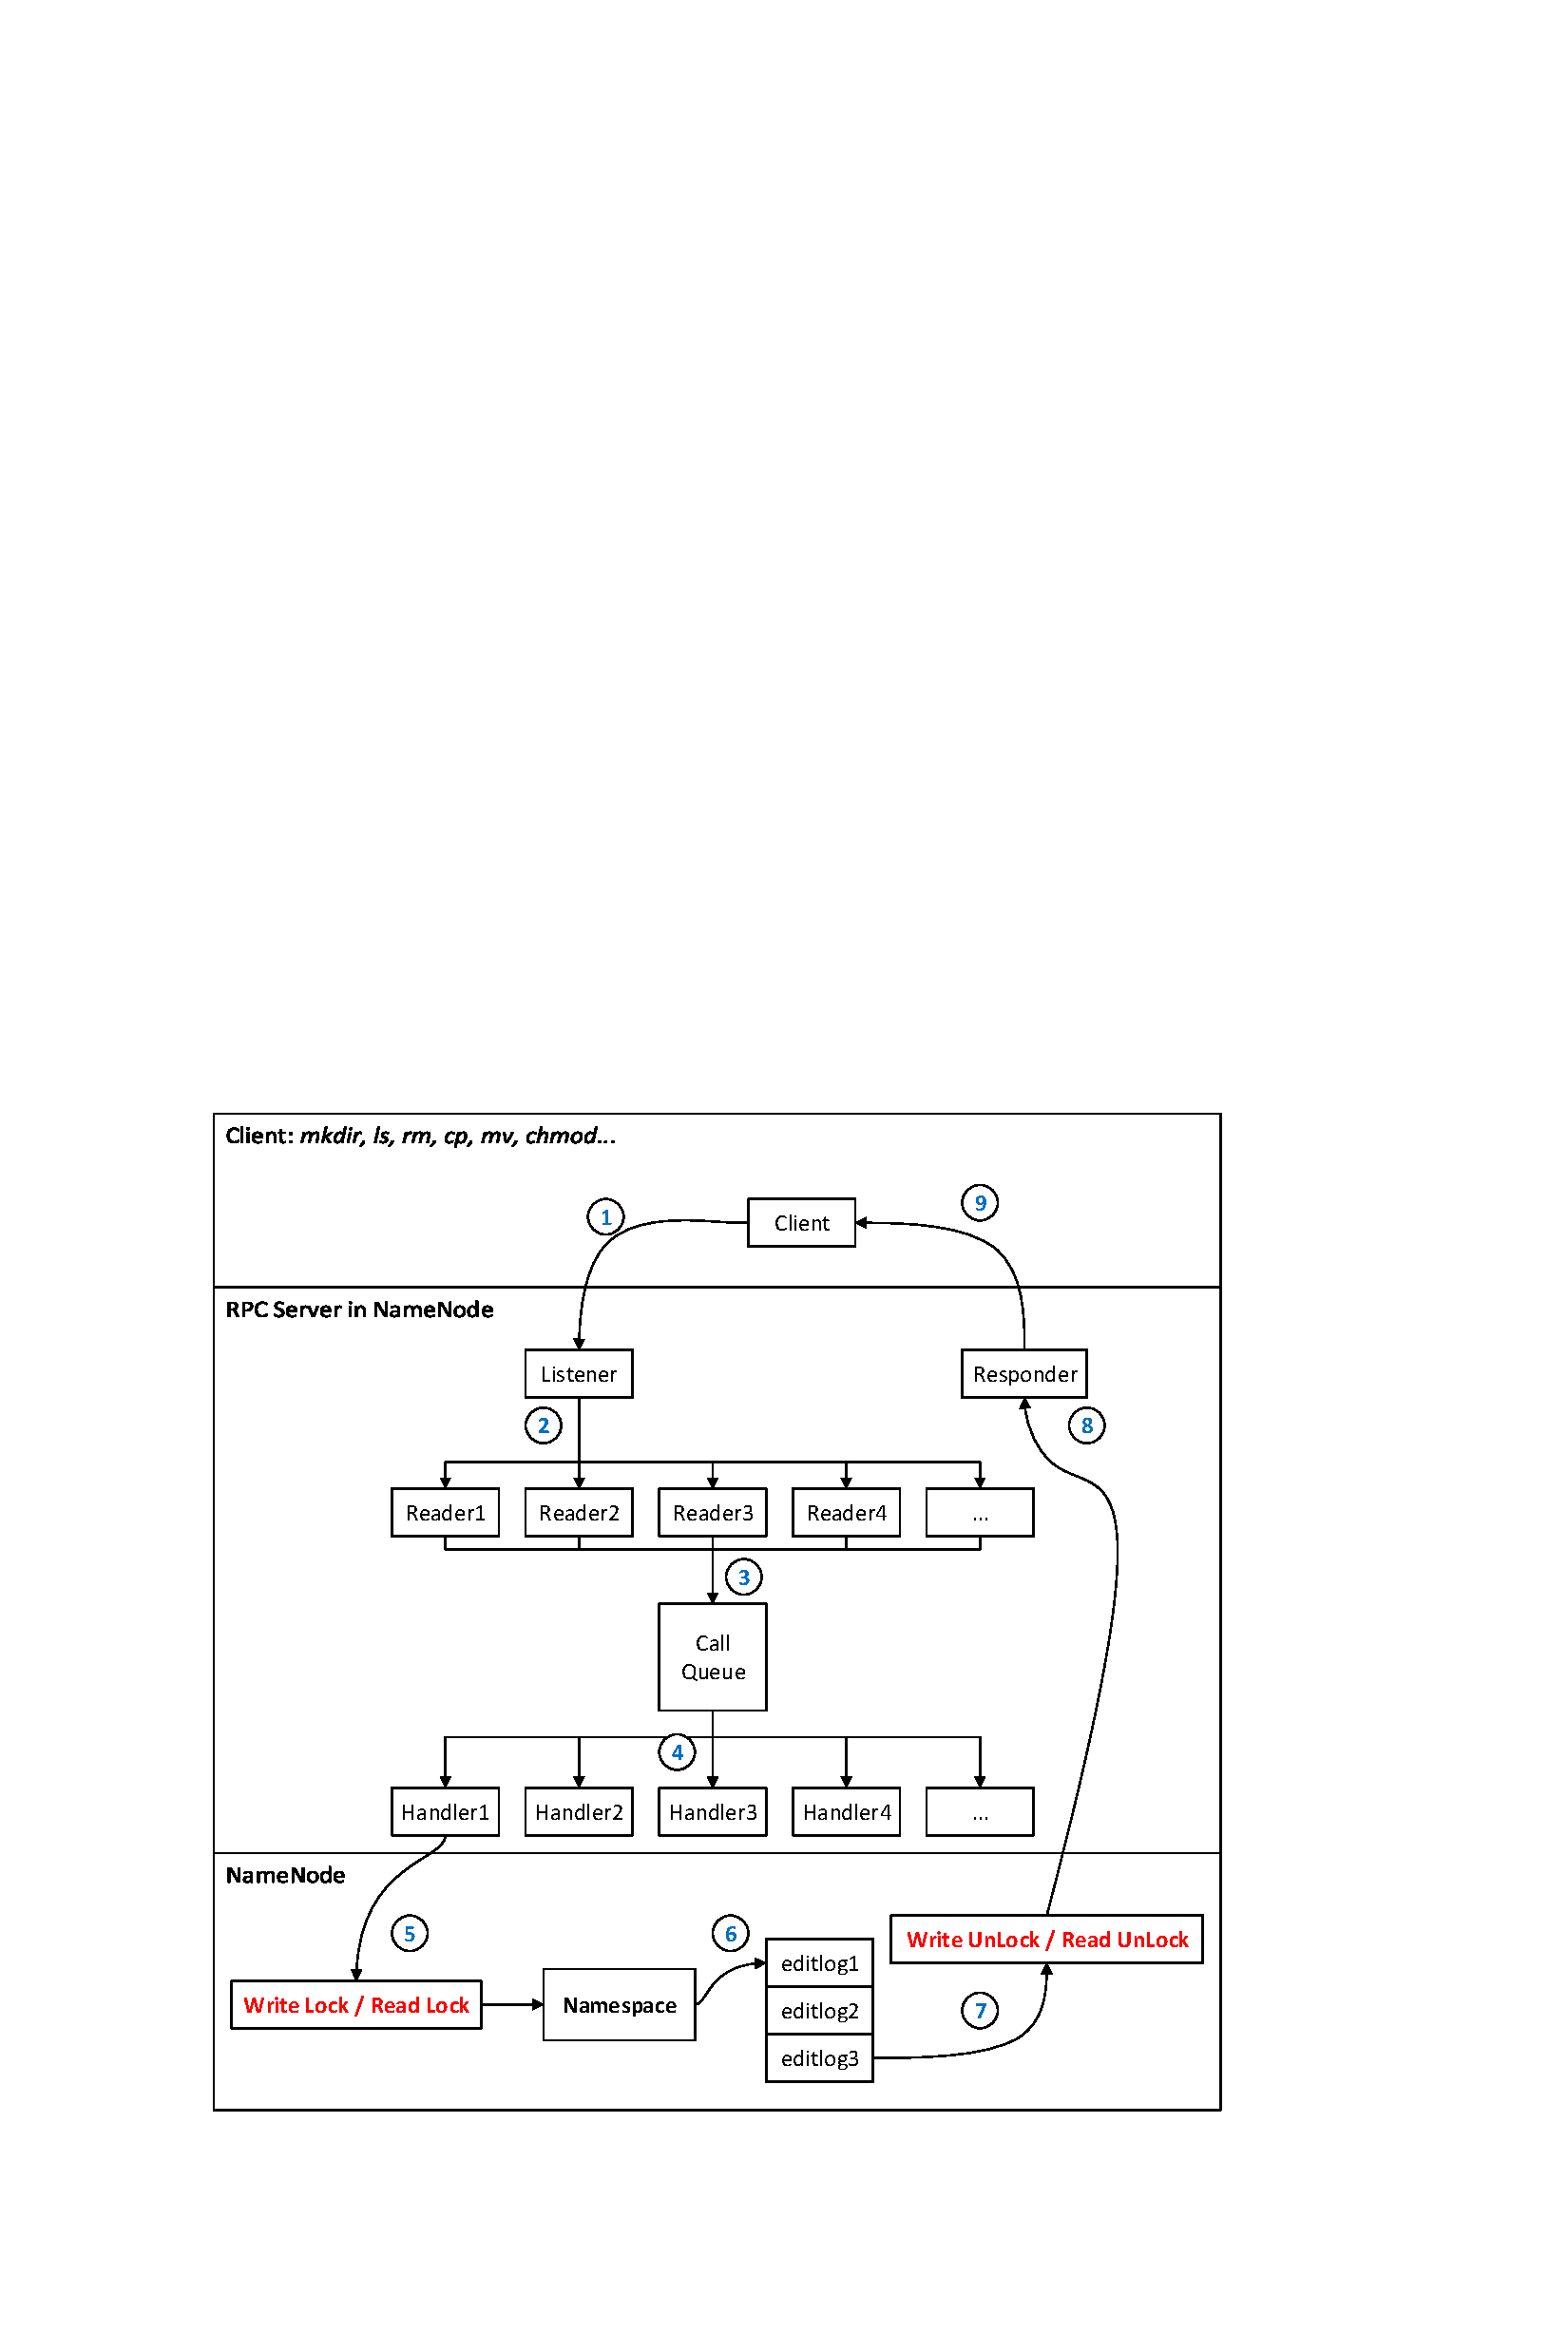
\includegraphics[scale=0.8]{figs/nnRPC.pdf}
	\caption{RPC between Clients and NameNode for Namespace Operations}
	\label{fig:nnRPC}
\end{figure}

  %%%%%%%%%%%%%%%%%%%%%%%%%%%%%%%%%%%%%%%%%%%%%%%%%%%%%%%%%%%%%%%%%%%%%%%%%%%%%
  %
%%%%%                      SECOND SECTION
 %%%
  %

\section{Namespace Concurrency Control in Hop-HDFS}

\subsection{Namespace Structure}
In HDFS, the namespace is kept in-memory as arrays and optimized data structure (like LinkedList) of objects with references for semantic constraints. Therefore, it has a \textit{directed tree structure}, similar to Figure~\ref{fig:gfsTree}. 

\noindent In Hop-HDFS, the namespace is stored into tables of MySQL Cluster database, so all INode objects are represented as individual row records in a single \textit{inodes table}. In order to preserve the directed tree structure, we add an id column and a parent\_id column to each row of in \textit{inodes table}. Therefore, the graphical representation of the filesystem hierarchy for INodes is like Figure~\ref{fig:hoptree}. The table representation in the database is like Table~\ref{table:hoptreeTable}.

\begin{figure}[h]
	\centering
	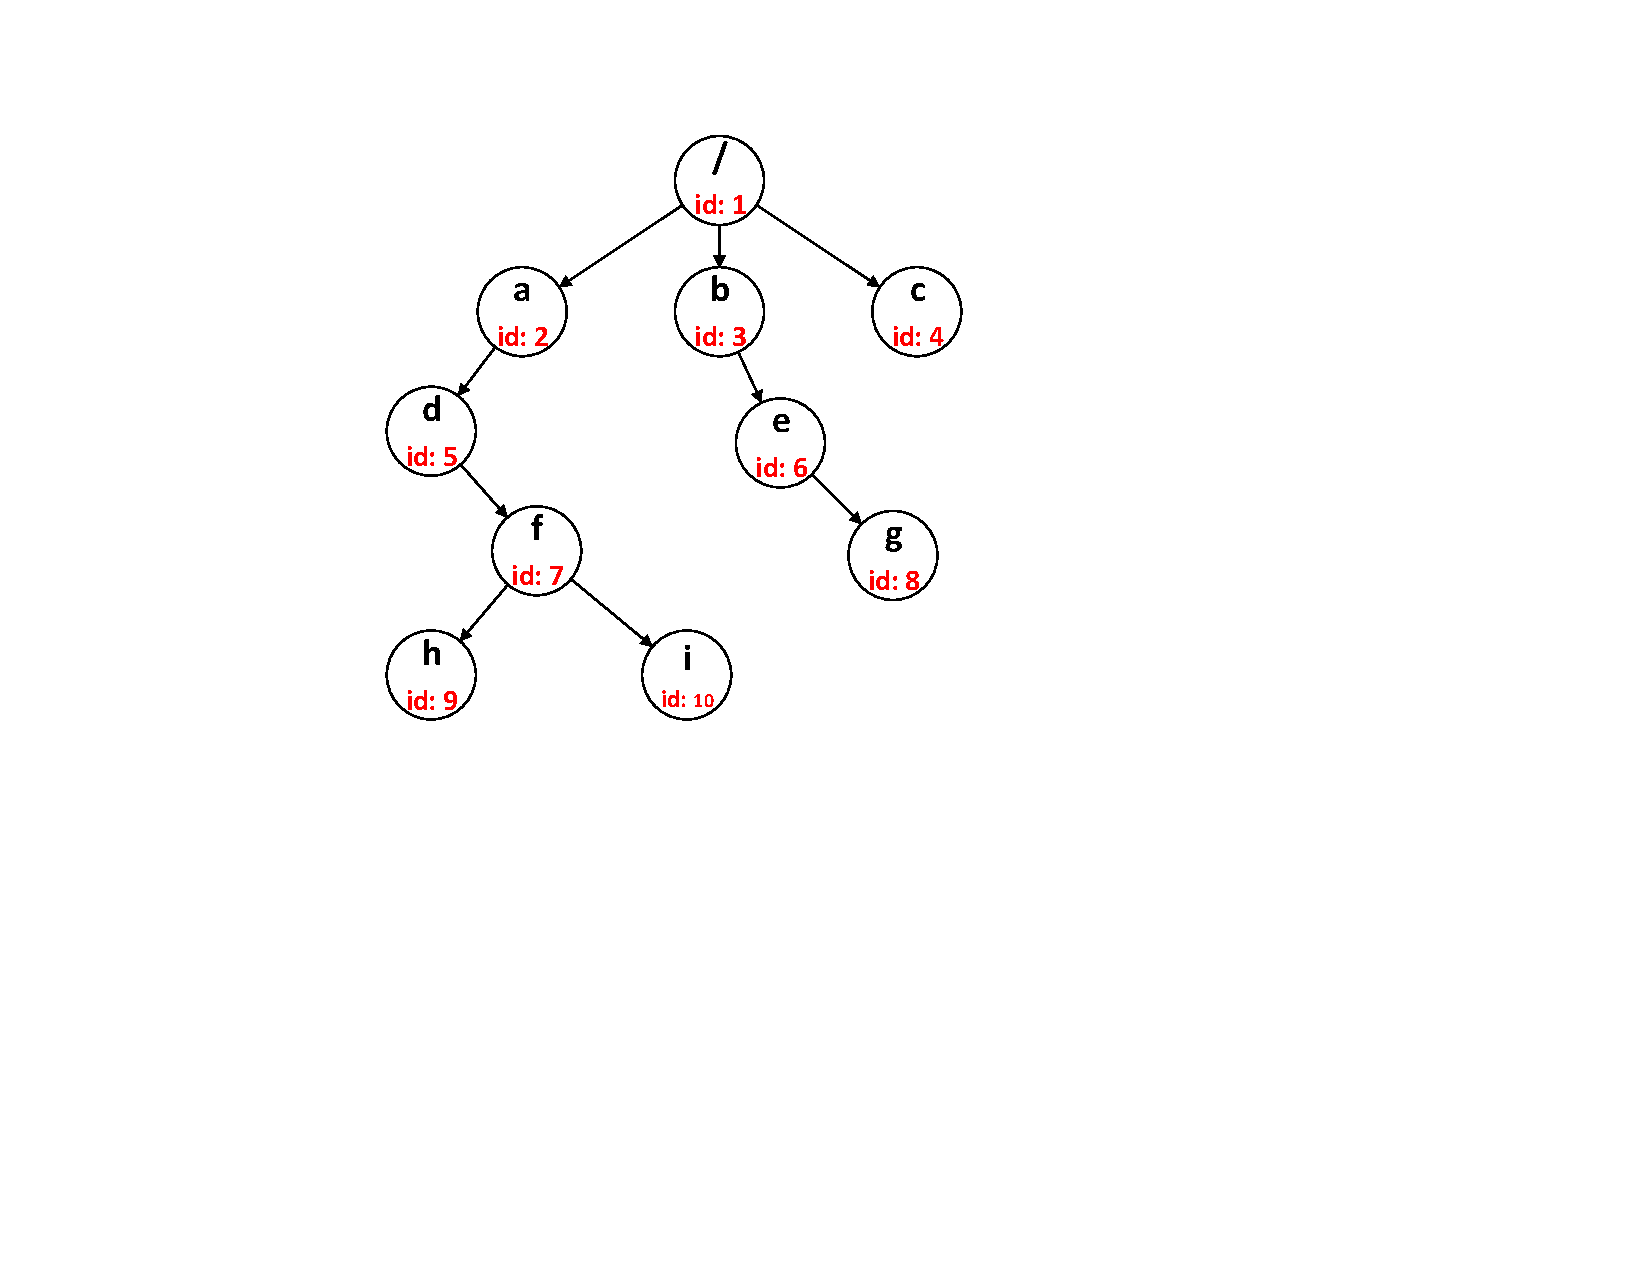
\includegraphics[scale=1]{figs/hoptree.pdf}
	\caption{Filesystem Hierarchy with ID for INodes in Hop-HDFS}
	\label{fig:hoptree}
\end{figure}

\begin{table}[h]
	\centering
	\begin{tabular}{|c|c|c|c|}
		\hline
		\textbf{id} & \textbf{parent\_id} & \textbf{name} & \textbf{other parameters...} \\ \hline
		1 & 0 & / & ... \\ \hline
		2 & 1 & a & ... \\ \hline
		3 & 1 & b & ... \\ \hline
		4 & 1 & c & ... \\ \hline
		5 & 2 & d & ... \\ \hline
		6 & 3 & e & ... \\ \hline
		7 & 5 & f & ... \\ \hline
		8 & 6 & g & ... \\ \hline
		9 & 7 & h & ... \\ \hline
		10 & 7 & i & ... \\ \hline
	\end{tabular}
	\caption{INode Table for Hop-HDFS}
	\label{table:hoptreeTable}
\end{table}

\noindent Since the \textit{id} is unique and atomically generated for INodes in each new transaction, the \textit{Primary Key} for the table is $<$name, parent\_id$>$ pair to avoid duplicated data rows during primary key lookup. With the \textit{id} and \textit{parent\_id} relationship, the hierarchy will be constructed correctly from the rows to be in-memory objects used by the name system.

\subsection{Namespace Concurrency Control}